\documentclass{article}

\usepackage[dblblindworkshop]{neurips_2026}
 % \usepackage[dblblindworkshop, final]{neurips_2026}

\workshoptitle{Workshop for Autonomous ML Research }

\usepackage[utf8]{inputenc}
\usepackage[T1]{fontenc}
\usepackage{url}
\usepackage{booktabs}
\usepackage{amsfonts}
\usepackage{nicefrac}
\usepackage{microtype}
\usepackage{xcolor}
\usepackage{graphicx}

\title{Hidden Consensus, Loud Disagreement: Autonomous ML Agents Diverge in What They
Measure but Converge on What They Conclude}

\author{%
  Anonymous Author(s) \\
  Anonymous Institution \\
  \texttt{anonymous@example.org} \\
}

\begin{document}

\maketitle

\begin{abstract}
Independent AI agents given identical machine
learning research questions and an identical dataset (UCI Adult/Census Income) diverge
sharply in what they choose to report when a question's operationalization is left
unspecified --- abstractly-worded questions produced 9.1 unique measure framings per 10
replicates on average across 120 independent, memory-isolated replicate analyses, versus
3.8 for concretely-specified questions. We show, however, that this surface-level divergence substantially overstates
genuine disagreement: on two abstract questions, replicates converge on the same
qualitative conclusion in 65--100\% of cases despite near-total disagreement on which
specific number to headline --- loud disagreement about what to report can coexist with
hidden consensus about what is true. We additionally test a domain-appropriate
intervention unavailable in prior (non-executable) research settings --- requiring agents
to verify their own finding via repeated cross-validation or bootstrap re-estimation
before reporting --- and find it does not reduce measure-choice diversity, but
appropriately tightens numeric estimates for robust effects while surfacing genuine
fragility in weak ones (sign agreement on a small effect drops from 90\% to 70\% once
agents are required to check it). A matching 120-replicate dataset collected with Claude
Haiku in place of Sonnet replicates these patterns, but also reveals a further failure
mode: on two hypotheses where both model families converge almost completely on
\emph{what} to measure, they reach opposite conclusions about \emph{what value they get}
(one effect reverses sign and grows 15$\times$ larger), traced to an upstream
preprocessing choice invisible in the measure name itself --- apparent consensus can mask
real disagreement just as easily as loud disagreement can mask real consensus. All
reported findings were independently verified via re-execution of each replicate's saved
analysis code against the original data: 208/240 (87\%) reproduced exactly or within
tolerance. The Sonnet dataset showed zero value mismatches; 4/120 Haiku replicates did,
traced to self-reported values not matching their own confirmed-deterministic code, a
distinct reliability gap we disclose in full.
\end{abstract}

\noindent\textbf{Keywords:} autonomous research, nonstandard errors, machine learning
evaluation, multi-agent verification, researcher degrees of freedom

\section{Autonomous research result}
This part is for the research itself: the hypothesis, method, evidence, and primary
result generated or developed by the agent.

\subsection{Hypothesis}

When independent human research teams are given the same dataset and question, they
routinely reach different quantitative conclusions --- not from error, but because the
space of defensible analytical choices (model, controls, metric, validation scheme) is
large, and different teams occupy different corners of it. \citet{menkveld2024} documented
this directly: 164 independent teams analyzing the same financial dataset produced
estimates whose disagreement --- ``nonstandard errors'' --- often rivaled or exceeded each
team's own reported statistical uncertainty. \citet{gaoxiao2026} recently showed
autonomous AI agents reproduce this: 150 independent Claude Code agents given the same six
market microstructure questions diverged sharply, driven by stable methodological forks,
with AI peer review largely failing to resolve the disagreement while exemplar exposure
did.

Both studies are confined to finance and social-science-style empirical analysis, where
the ``correct'' measure is inherently a matter of judgment rather than something
executable and checkable --- unlike machine learning research, whose central operations
(train a model, evaluate it, compute a metric) are directly checkable. This raises two
questions neither prior study could address: does the same nonstandard-errors phenomenon
appear when the domain provides mechanical ground truth, and, because ML tasks are
executable, does asking agents to verify their own findings by re-running the analysis
under a stability check reduce disagreement the way exemplar exposure did for Gao and Xiao
--- an intervention with no clean analogue where the underlying ``truth'' cannot itself be
re-executed?

We hypothesize that (H-a) measure-choice divergence replicates in the ML domain, driven
primarily by whether a question's operationalization is specified, and (H-b)
self-verification reduces numeric uncertainty in a chosen measure without resolving
disagreement about which measure to choose. H-a predicts higher measure-framing diversity
for abstract than concrete questions; H-b predicts the verification arm changes numeric
dispersion/sign agreement without changing measure-choice diversity.

\subsection{Method}

\textbf{Dataset.} All replicates analyze a single, static copy of the UCI/OpenML Adult
(Census Income) dataset (48{,}842 rows, mixed categorical/numeric features, binary income
target, ${\sim}$24\% positive class), fetched once and frozen so every replicate receives
byte-identical data.

\textbf{Research questions.} We wrote six research questions about this dataset, in three
matched abstract/concrete pairs (Table~\ref{tab:hypotheses}). Each replicate agent
receives only the dataset and one research question --- no documentation, no access to any
other replicate's work, and no information about which other measures might be
reasonable.

\begin{table}[h]
  \caption{The six research questions, in three abstract/concrete matched pairs.}
  \label{tab:hypotheses}
  \centering
  \small
  \begin{tabular}{p{0.04\linewidth}p{0.12\linewidth}p{0.72\linewidth}}
    \toprule
    ID & Specificity & Question \\
    \midrule
    H1 & Abstract & Does model family meaningfully affect predictive performance? \\
    H2 & Concrete & Does default-hyperparameter random forest beat default logistic
    regression on stratified 5-fold CV ROC-AUC? \\
    H3 & Abstract & Which features are most important for predicting income? \\
    H4 & Abstract & Does addressing class imbalance improve model quality? \\
    H5 & Concrete & Does SMOTE oversampling change minority-class F1 by more than 0.02
    versus no resampling, holding the classifier fixed? \\
    H6 & Abstract & Is the model well-calibrated? \\
    \bottomrule
  \end{tabular}
\end{table}

\textbf{Isolation and scale.} Every replicate runs as an independent, non-interactive
Claude Code CLI invocation (\texttt{claude -p ... --dangerously-skip-permissions}) in a
freshly created, unpredictably-named temporary directory with no persistent sibling
directories visible at any point, and an explicit instruction not to explore outside its
own working directory. We collected 10 independent replicates per (hypothesis $\times$
arm) cell --- 120 replicates total with Claude Sonnet, plus a matching 120-replicate
cross-model-family check with Claude Haiku (Section~\ref{sec:research-loop}).

\textbf{The verification arm.} Half of the replicates for each hypothesis (the ``verify''
arm) receive an additional instruction: before reporting, validate your finding's
stability via repeated cross-validation with different seeds, a bootstrap confidence
interval, or a held-out re-test split, and report whether it held up. The other half
(``no-verify'') report directly after a single analysis pass.

\textbf{Structured reporting.} Every replicate writes a structured result (a named metric,
its value, a direction, and free-text on its methodological choices) rather than a forced
common statistical form, since abstract questions admit incompatible units.

\textbf{Verification of our own data.} Independent of the verification \emph{arm}, we
re-executed every replicate's saved code against fresh data: 208/240 (87\%) reproduced.
Sonnet showed zero contradicting values; 4/120 Haiku replicates did, traced to
self-reports not matching their own deterministic code (Section~\ref{sec:verification}).

\subsection{Evidence}

\textbf{Measure-choice diversity tracks abstractness.} Figure~\ref{fig:diversity} shows
the number of distinct measure framings (collapsing trivial rewordings into one canonical
form) each hypothesis produced across 20 replicates. The contrast is stark: H2 (concrete)
produced only 2 distinct framings, essentially all rewordings of ``ROC-AUC difference (RF
$-$ LogReg)''; its abstract counterpart H1 produced 15. H5 (concrete) produced 10; H4
(abstract) produced 19. H3 and H6, abstract questions with an implicit but unstated
method, land in between (15 and 17): agents agreed on \emph{method} (permutation
importance; 10-bin ECE) while diverging on \emph{target}. Collapsed into abstract vs.\
concrete, this is a 2.4$\times$ difference in mean unique framings (9.1 vs.\ 3.8 per 10)
and 3.6$\times$ in how much the modal framing dominates (19\% vs.\ 68\%).

\begin{figure}[h]
  \centering
  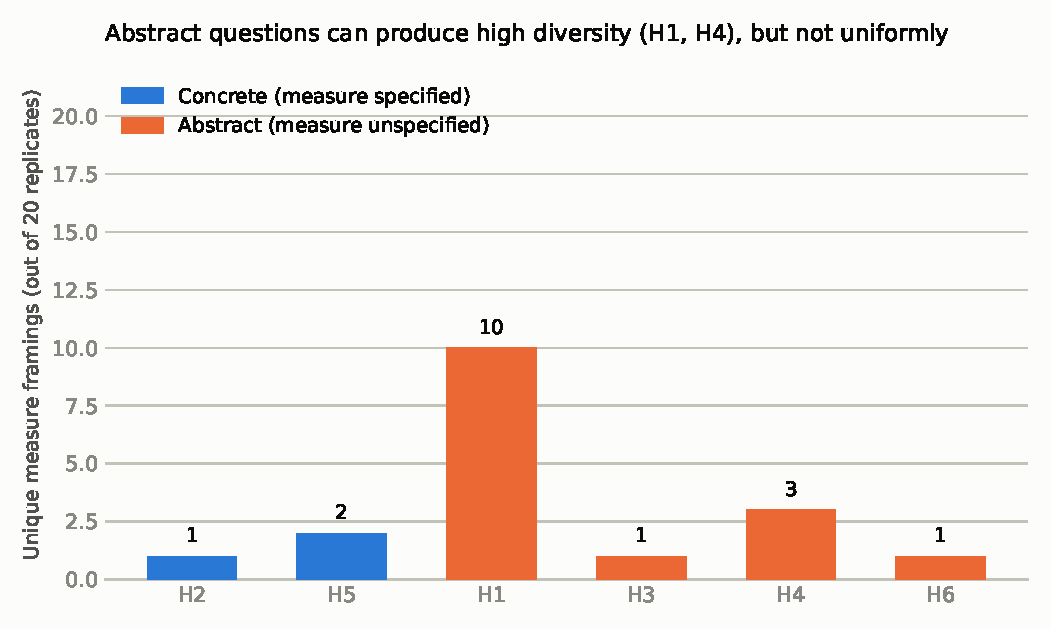
\includegraphics[width=0.85\linewidth]{fig1_diversity.pdf}
  \caption{Unique measure framings per hypothesis (out of 20 replicates, 10 per arm).
  Concrete questions (blue) converge on a small number of framings; abstract questions
  (orange) produce near-total diversity.}
  \label{fig:diversity}
\end{figure}

\textbf{Surface disagreement overstates substantive disagreement.} The diversity counts
above, read alone, would suggest near-total disagreement on abstract questions --- too
strong a conclusion. For H1, 20/20 replicates (100\%) agreed a tree-ensemble model
(Gradient Boosting, HistGradientBoosting, or Random Forest) outranks linear/naive
baselines, despite zero agreement on which pair to headline. For H4, 13/20 (65\%)
explicitly stated the full pattern ``balanced accuracy/minority recall improves, ROC-AUC
stays roughly flat''; 18/20 (90\%) agreed at minimum on ``improves,'' despite 19/20 unique
framings.

\textbf{Verification changes numeric confidence, not measure choice.}
Figure~\ref{fig:verifyarm} compares the no-verify and verify arms for H2 and H5. For H2 ---
a large, robust effect --- sign agreement is 100\% in both arms, and verification tightens
the spread (SD 0.0038 $\rightarrow$ 0.0022). For H5 --- small and fragile --- sign
agreement \emph{falls} under verification, 90\% $\rightarrow$ 70\%, and the mean effect
shrinks toward zero ($-0.0028 \rightarrow -0.0016$): several verify-arm replicates that saw
an effect on one split found, once checked via repeated CV, that the sign was unstable
across folds, and reported this explicitly.

\begin{figure}[h]
  \centering
  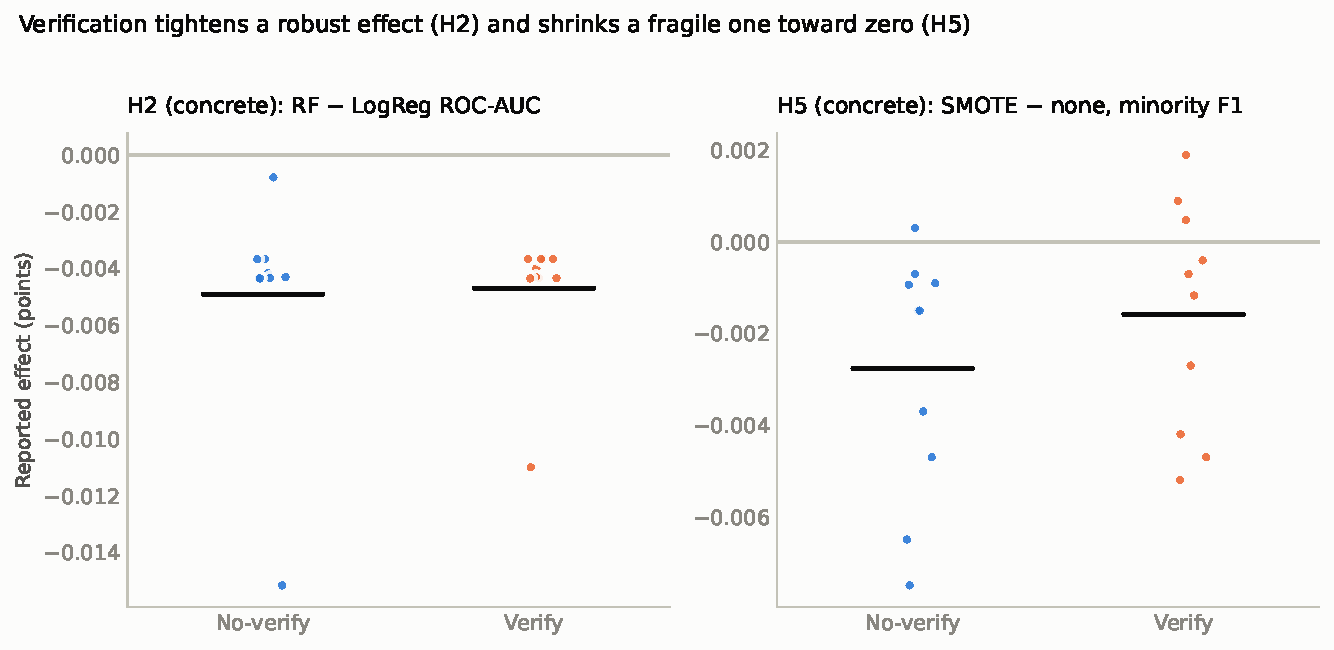
\includegraphics[width=0.95\linewidth]{fig2_verify_arm.pdf}
  \caption{Replicate-level values for H2 and H5 by arm. Verification tightens a robust
  effect (H2) and shrinks a fragile one toward zero (H5); black bars show arm means.}
  \label{fig:verifyarm}
\end{figure}

\textbf{A cross-model-family check surfaces hidden disagreement despite apparent
consensus.} The core patterns replicate with Haiku in place of Sonnet: unique framings
remain higher for abstract than concrete questions (Table~\ref{tab:crossmodel}), and H1's
substantive convergence holds (18/20 Haiku vs.\ 20/20 Sonnet agree a tree ensemble wins)
--- though the gap's size varies and even reverses for H6, where Haiku converged more (5
vs.\ 17). More strikingly, H2 and H5 --- where both models agree almost completely on
\emph{what} to measure --- reverse on \emph{what value they get}: Sonnet unanimously finds
logistic regression beating random forest on H2 (mean $-0.0049$); 90\% of Haiku replicates
find the opposite, 15$\times$ larger (mean $+0.0765$), traced to Haiku disproportionately
using naive label-encoding where Sonnet one-hot encoded --- invisible in the measure name
itself. This is close to the mirror image of our main finding: not loud disagreement
masking hidden consensus, but apparent consensus masking real disagreement.

\begin{table}[h]
  \caption{Cross-model-family diversity: unique canonical measure framings per hypothesis
  (out of 20 replicates, both arms combined).}
  \label{tab:crossmodel}
  \centering
  \small
  \begin{tabular}{lccc}
    \toprule
    Hypothesis & Specificity & Sonnet & Haiku \\
    \midrule
    H1 & Abstract & 15 & 17 \\
    H2 & Concrete & 2 & 1 \\
    H3 & Abstract & 16 & 19 \\
    H4 & Abstract & 19 & 20 \\
    H5 & Concrete & 10 & 15 \\
    H6 & Abstract & 17 & 5 \\
    \bottomrule
  \end{tabular}
\end{table}

\subsection{Primary Result}

Across six machine learning research questions and 240 independent, memory-isolated agent
replicates (120 Sonnet, 120 Haiku): (1) question specificity is, as in prior non-ML
domains, the primary driver of agent-to-agent disagreement, extending nonstandard errors
in AI-conducted research \citep{gaoxiao2026,menkveld2024} into the one domain their method
could not reach; (2) this surface-level divergence overstates genuine disagreement, with
substantive conclusions converging in 65--100\% of cases despite near-total disagreement on
what to report; (3) self-verification recalibrates numeric confidence without touching
measure-choice diversity, tightening robust effects and surfacing fragile ones; and (4)
these patterns replicate across model families, but agreement on \emph{what} to measure
does not guarantee agreement on the value obtained --- a second model family can reverse a
unanimous finding entirely. Results (3)--(4) jointly show how ``self-verification'' should
be read as a mitigation: it targets estimation noise in an already-chosen measure, with no
mechanism to resolve disagreement about which measure was right, or what a different agent
would have found.

\clearpage
\section{System Design and Meta-Analysis}
This is a human-author companion to the main result and should act as a meta-analysis of
the research process undertaken.

\subsection{Agent and Harness}

All experimental replicates were produced by Claude Sonnet, invoked through the standalone
Claude Code CLI (\texttt{@anthropic-ai/claude-code}, v2.1.221) rather than through the
Anthropic API directly, using the author's existing subscription rather than separate
metered billing. Each replicate is a single, non-interactive invocation ---
\texttt{claude -p "<brief>" --dangerously-skip-permissions --model sonnet} --- run with its
working directory set to a freshly created, unpredictably-named temporary directory
containing only a static copy of the dataset. \texttt{--dangerously-skip-permissions} was
necessary for unattended batch execution across well over a hundred replicate runs, a real
reduction in interactive safety guardrails relative to normal Claude Code use.

Isolation between replicates was approximated at two levels: a fresh, non-shared
filesystem location per replicate, and an explicit brief instruction not to read, list, or
explore any directory other than the replicate's own working directory. This is weaker
than the container/Singularity-based isolation used in the most directly comparable prior
work \citep{gaoxiao2026}, which reports having observed agents reading sibling outputs
without such isolation during their own trial runs; we did not build container-level
isolation for this laptop-scale study (Section~\ref{sec:limitations}).

Every replicate was asked to produce a structured result file (a named primary metric, its
value, a qualitative direction, and free-text methodological-choices text) plus its
analysis code as a saved script, avoiding the unit-normalization problem
\citet{gaoxiao2026} had to solve after data collection by asking each agent to self-report
one named metric and its own reasoning rather than forcing a common statistical form up
front.

\subsection{Tools}

The agent's own toolset within each replicate session was the standard Claude Code toolset
(file read/write, bash execution) with no additional MCP servers or external tools
configured; agents wrote and executed their own Python analysis code, predominantly using
scikit-learn, pandas, and, for several replicates addressing class imbalance,
imbalanced-learn/SMOTE. The orchestrating batch harness --- dispatching replicates,
managing isolation, collecting results, and the later verification and analysis passes ---
was written in Python using standard scientific-Python tooling
(\texttt{concurrent.futures}, pandas, scikit-learn, matplotlib), run locally with no cloud
infrastructure beyond the Claude Code CLI calls themselves. All experiments ran on a
single Apple Silicon laptop with no dedicated GPU or compute cluster. Total data
collection spanned roughly 33 calendar hours across five retry waves, but only about 3--4
of those hours involved any replicate actively running; the remainder was idle time between
waves, reflecting both the CLI's session usage limit and whenever the human author was
next available to check and relaunch collection (Section~\ref{sec:research-loop}).

\subsection{Research Loop}
\label{sec:research-loop}

The research loop had three phases: topic selection, data collection, and analysis.

\textbf{Topic selection} involved an extended, iterative novelty-checking process: roughly
fifteen candidate research questions across three genres (LLM agent behavior/reliability;
classical ML mechanisms; large-scale systematic ML audits) were proposed and checked
against current literature via web search, and the great majority were found to already
have close prior art, in several cases published within weeks of the check. The direction
pursued here was arrived at only after an earlier framing was found to substantially
overlap with \citet{gaoxiao2026} and an adjacent cluster of very recent work, prompting a
search for a structurally, not just incidentally, distinct angle: the ML domain those
studies could not reach.

\textbf{Data collection} proceeded in waves rather than a single pass. During batch
execution, the harness repeatedly encountered the Claude Code CLI's session usage limit;
since each replicate's result is logged independently, the harness resumed by re-running
only cells without a completed replicate, so already-completed runs were never discarded.
This required five separate retry waves spanning roughly 33 calendar hours, though only
about 3--4 hours of that involved any replicate actively running --- the rest was idle time
between waves, reflecting both the session limit itself and when the human author was next
available to check and relaunch collection. The practical per-window ceiling turned out to
be far smaller and more variable (roughly 15--56 successful heavy-agentic runs per window)
than anticipated. Collection also surfaced a
genuine failure mode: a subset of replicates --- disproportionately the more compute-heavy
verification-arm ones --- were found to spawn their analysis as a background shell task and
then end their turn waiting for a completion notification that could never arrive in a
single-shot, non-interactive session. An explicit instruction against this was added to
the brief template; it measurably reduced but did not eliminate the failure mode. A
separate lifecycle issue --- three replicate slots that each succeeded twice under
different run identifiers, traced to an orchestration process being halted without
terminating its already-spawned subprocesses --- was resolved by keeping the
earlier-started run of each pair, a rule fixed before any outcome was inspected. The
dataset was finally trimmed to a uniform N=10 replicates per cell (120 total) by
restricting to a fixed replicate-index range in every cell, a rule fixed at dispatch time
for presentational clarity.

\textbf{Analysis} proceeded through iterative drafting, figure generation, and review,
detailed further in Section~\ref{sec:human-interventions}.

\subsection{Human Interventions}
\label{sec:human-interventions}

The human author made every scope decision throughout the loop described in
Section~\ref{sec:research-loop}: rejecting an initial research direction once it was found
to overlap with recent prior art and directing the agent toward the ML-domain extension;
choosing the execution mechanism (CLI over a raw API key) and model-family scope (single
family, deferred rather than abandoned); setting and later defending the replicate count
(N=10 per cell) against a further reduction to N=5 that the agent had not proposed but the
human considered and overruled on statistical grounds, since the verification-arm
comparison --- the paper's most novel manipulation --- would have had too little power at
that sample size; and reviewing drafted figures and text at each stage. During review, the
human author caught a specific framing problem the agent had not flagged on its own: an
early draft title reused a precursor paper's exact title as a substring, which would have
read as a derivative reskin before a reader reached the abstract; the title was changed to
lead with this paper's own distinctive contribution instead. The human author also set the
boundary that all reported figures (including replicate counts and the record of process
incidents in this section) must reflect what actually happened, rather than a
retrospectively cleaner narrative, and that this section's substantial drafting
collaboration with the agent be disclosed rather than presented as solely human-authored
--- consistent with, and enforcing, this workshop's disclosure policy.

\subsection{Verification}
\label{sec:verification}

Two distinct verification mechanisms appear in this paper and should not be conflated. The
\textbf{verification arm} is an experimental manipulation under study (Section~1.3), not a
claim about data quality. Separately, we independently verified the \textbf{correctness of
the underlying dataset} by re-executing every replicate's saved analysis code against a
fresh copy of the source data and comparing the reproduced primary metric to the one
originally reported --- a check made possible, and cheap, by the fact that ML analyses are
directly executable, unlike the empirical-finance analyses in the most comparable prior
work.

For the primary Sonnet dataset, 113 of 120 replicates (94\%) reproduced exactly or within
small numerical tolerance, and zero replicates showed a script running to completion and
producing a value that contradicted its own report; every discrepancy traced to a
limitation of the re-verification method itself (a timeout on the heaviest
verification-arm scripts, and a smaller number of replicates whose saved script was not
fully self-contained).

Running the same check on the Haiku dataset surfaced a different and more concerning
pattern: 95 of 120 replicates (79\%) reproduced, and this time 4 replicates' saved scripts
ran to completion and produced a value that contradicted their own report. We manually
re-ran a sample of these mismatching scripts twice each and confirmed they are fully
deterministic (identical output both times), ruling out simple run-to-run non-determinism;
the discrepancy is instead between what the agent's saved code actually computes and what
it self-reported, which for these replicates were apparently produced independently rather
than the report being derived from that code's own execution. The remaining 21
non-reproducing Haiku replicates match the same not-self-contained-script pattern seen in
Sonnet, at a notably higher rate (17.5\% vs.\ 5\%).

We disclose all of this plainly: re-execution establishes that reported numbers were not
fabricated on the runs it could fully check and confirm, but it also surfaced --- rather
than merely failed to rule out --- a real, model-family-specific self-report reliability
gap. This is itself consistent with this paper's main finding: verification is not one
thing, and a check aimed at one failure mode (fabrication) can, run rigorously enough,
catch a different one (self-report/execution inconsistency) it was not specifically
designed to find.

\subsection{Significance of result}

The result matters for two different audiences. For researchers using AI agents as
empirical collaborators, it is a direct, actionable warning: an underspecified request to
an AI agent does not fail loudly, it fails quietly, by returning a confident, well-argued
answer to a question subtly different from the one intended --- and the fix demonstrated
here (specifying the measure, not just the goal) is cheap and available today. For the
autonomous-research community this workshop represents, the more important result may be
the second one: that a verification step targeting numerical stability does not, and
structurally cannot, resolve disagreement about what to measure in the first place. As
autonomous agents are given more latitude in real research pipelines, ``have the agent
check its own work'' is a natural first line of defense; this result suggests that defense
has a specific, identifiable blind spot, and that closing it likely requires a different
kind of intervention (in the spirit of the exemplar-exposure result of \citet{gaoxiao2026})
rather than a more thorough version of the same one.

\subsection{Interpretability}

All experimental artifacts were tracked to support post-hoc audit. Every replicate's raw
result, saved analysis code, and run metadata (timing, success/failure status, verification
outcome) were written to a dedicated, per-run directory identified by a unique run ID.
Every batch dispatch and retry wave was logged, one line per attempt, to an append-only
log recording hypothesis, arm, replicate index, and outcome, so the full history of
successes, failures, retries, and duplicates is independently reconstructable rather than
overwritten. Excluded and superseded runs (failed attempts, and duplicate successes
resolved during data cleaning) were archived rather than deleted and remain available for
inspection. Separately from the experimental logs, a chronological process log recording
every scope decision, incident, and its resolution was maintained throughout the project
and is available as supplementary material; Section~\ref{sec:research-loop} and
Section~\ref{sec:human-interventions} are drawn directly from it.

\subsection{Limitations}
\label{sec:limitations}

Isolation between replicates is prompt-level and filesystem-layout-based, not an OS-level
sandbox guarantee; we cannot rule out imperfect isolation in ways container-based isolation
would have prevented, though we have no direct evidence of cross-contamination in our
data. This study covers two model families (Sonnet, Haiku; Section~1.3); broader coverage
(e.g.\ Opus, or non-Anthropic families) was not attempted, and unlike the primary Sonnet
dataset, the Haiku dataset's re-verification (Section~\ref{sec:verification}) was run as a
follow-up check rather than alongside initial collection. N=10 replicates per cell is well
below the 150 used in the most
comparable prior study, sized for laptop/subscription-quota feasibility rather than by
power analysis. Our re-verification of replicate outputs, while extensive, could not fully
check every replicate's process end-to-end, for the reasons given in
Section~\ref{sec:verification}.

\clearpage
\section{Reflections and Broader Impact}

This paper's main practical implication is a warning with an inverted risk profile from
the usual failure mode people worry about with autonomous agents: the danger here is not
that an agent visibly fails, but that it succeeds confidently and quietly at a slightly
different task than intended, in a way that is only detectable by comparing many
independent attempts. As autonomous agents take on a larger share of applied ML work ---
model selection, feature engineering, evaluation design --- this failure mode will mostly
go unnoticed by a single researcher running a single analysis, since nothing about a lone
run signals that a different, equally defensible choice existed. The positive implication
is equally direct: this risk is cheap to mitigate. Specifying the measure, not just the
goal, collapsed measure-choice diversity by roughly $2.4\times$ in our data, at zero
additional cost. We would encourage practitioners delegating open-ended ML analysis to
agents to treat explicit measure specification as a default, not an afterthought.

For this workshop's broader question of how the field should adapt, we would highlight two
points beyond this paper's specific result. First, our own novelty-checking process ---
roughly fifteen candidate directions checked against current literature, the great
majority already covered by work published within weeks --- suggests that ``we searched
and found nothing'' is weakening as evidence of novelty specifically for autonomous
research submissions, since the same tools that accelerate one group's research loop
accelerate everyone else's. Venues may need to treat rapid, independent convergent
discovery as an expected feature of the genre rather than a sign that a submission was
insufficiently diligent. Second, self-verification is not one thing: this paper required
two structurally different verification steps (an experimental manipulation testing
whether agents checking their own numerical stability changes what they report, and an
independent check that reported numbers were not fabricated), and conflating them would
have been easy to do by accident. As ``have the agent check its own work'' becomes a
standard mitigation for autonomous-agent unreliability, we would encourage reviewers and
discussants to ask specifically which kind of wrongness a given verification step could
and could not have caught, rather than treating any plausible-sounding check as covering
all of them. Third, a laptop and a subscription are not yet a research lab, and the gap is
measurable: this paper's 120 replicates needed roughly 33 calendar hours and five retry
waves despite only 3--4 hours of active computation (Section~2.3) --- an artificial usage
cap, not compute capability, where the most comparable prior study ran 150 agents against
metered billing with no such wall \citep{gaoxiao2026}. Access to a research lab
increasingly means access to a \emph{budget}, which shapes which questions are practically
askable, not just how quickly they get answered --- worth this workshop's attention, since
it bears on who gets to participate in autonomous research at all.

We do not see meaningful negative societal impact specific to this work: it uses a
standard public benchmark dataset, introduces no new model or capability, and its
practical recommendation (specify measures explicitly) reduces rather than increases risk
from autonomous-agent-driven research.

\clearpage
\appendix

\section{Reproducibility Statement}

The dataset (UCI/OpenML Adult/Census Income) is public and freely available. The six
research questions are given in full in Table~\ref{tab:hypotheses}; the exact brief text
given to each replicate agent, including the verification-arm instruction, is available as
supplementary material. Reproducing the replicate-collection process requires the Claude
Code CLI and access to Claude Sonnet and Claude Haiku under the same or comparable
versions; because model
behavior can drift across versions, we do not expect bit-exact reproduction of individual
replicate outputs, but do expect the qualitative pattern (higher measure-choice diversity
for abstract questions; verification tightening robust effects and surfacing fragile ones)
to be checkable by any lab with CLI access to a comparable agent. All analysis code
(harness, verification, figure generation) is standard Python/scikit-learn and is included
in supplementary material along with the full experimental log described in
Section~\ref{sec:research-loop}. \emph{[Author note: confirm final code/data hosting
location --- e.g., an anonymized repository --- before submission, and update this
statement with the access details.]}

\section{Disclosure Statement}

\paragraph{Agent(s) / model(s) used} Claude Sonnet and Claude Haiku, via the Claude Code
CLI (\texttt{@anthropic-ai/claude-code} v2.1.221). The agent conducted all 240 experimental
replicates (120 Sonnet, 120 Haiku: data analysis, code writing and execution, result
reporting) as described in Section~1--2, and substantially assisted in drafting this
paper, including Section~1 in full and a first draft of Section~2, subsequently reviewed,
corrected, and revised by the human author as described in
Section~\ref{sec:human-interventions}.

\begin{itemize}
  \item[$\square$] A human author has curated this work and verified every claim,
    figure, methodology detail, and reference.
  \item[$\square$] A human author takes full accountability for the submission as
    a human-authored, human-verified artifact.
\end{itemize}

\emph{[Author note: check both boxes only once you have personally verified every claim,
figure, and reference below --- do not check these before that review is actually done.]}

\bibliographystyle{plainnat}
\begin{thebibliography}{9}

\bibitem[Gao and Xiao(2026)]{gaoxiao2026}
Ruijiang Gao and Steven Chong Xiao.
\newblock Nonstandard errors in AI agents.
\newblock \emph{arXiv preprint arXiv:2603.16744}, 2026.

\bibitem[Menkveld et~al.(2024)]{menkveld2024}
Albert~J. Menkveld, Anna Dreber, Felix Holzmeister, Juergen Huber, Magnus Johannesson,
Michael Kirchler, Michael Razen, Utz Weitzel, et~al.
\newblock Nonstandard errors.
\newblock \emph{The Journal of Finance}, 79(3):2339--2390, 2024.

\end{thebibliography}

\section*{NeurIPS Paper Checklist}

\begin{enumerate}

\item {\bf Claims}
    \item[] Question: Do the main claims made in the abstract and introduction accurately reflect the paper's contributions and scope?
    \item[] Answer: \answerYes{}
    \item[] Justification: The claims in the abstract are restated precisely in Section~1.4
    (Primary Result) and supported by the evidence in Section~1.3; the abstract states the
    qualifying result explicitly (measure-choice diversity by question specificity, the
    surface-vs-substance distinction, and the verification-arm asymmetry) as required by
    this workshop's eligibility rules.
    \item[] Guidelines:
    \begin{itemize}
        \item The answer \answerNA{} means that the abstract and introduction do not include the claims made in the paper.
        \item The abstract and/or introduction should clearly state the claims made, including the contributions made in the paper and important assumptions and limitations. A \answerNo{} or \answerNA{} answer to this question will not be perceived well by the reviewers. 
        \item The claims made should match theoretical and experimental results, and reflect how much the results can be expected to generalize to other settings. 
        \item It is fine to include aspirational goals as motivation as long as it is clear that these goals are not attained by the paper. 
    \end{itemize}

\item {\bf Limitations}
    \item[] Question: Does the paper discuss the limitations of the work performed by the authors?
    \item[] Answer: \answerYes{}
    \item[] Justification: Section~2.8 discusses isolation guarantees (prompt-level, not
    OS-level), the two-model scope (broader coverage not attempted), sample size
    (N=10 per cell, well below the most comparable prior study's 150), and the documented
    limits of our re-execution verification method (Section~2.5).
    \item[] Guidelines:
    \begin{itemize}
        \item The answer \answerNA{} means that the paper has no limitation while the answer \answerNo{} means that the paper has limitations, but those are not discussed in the paper. 
        \item The authors are encouraged to create a separate ``Limitations'' section in their paper.
        \item The paper should point out any strong assumptions and how robust the results are to violations of these assumptions (e.g., independence assumptions, noiseless settings, model well-specification, asymptotic approximations only holding locally). The authors should reflect on how these assumptions might be violated in practice and what the implications would be.
        \item The authors should reflect on the scope of the claims made, e.g., if the approach was only tested on a few datasets or with a few runs. In general, empirical results often depend on implicit assumptions, which should be articulated.
        \item The authors should reflect on the factors that influence the performance of the approach. For example, a facial recognition algorithm may perform poorly when image resolution is low or images are taken in low lighting. Or a speech-to-text system might not be used reliably to provide closed captions for online lectures because it fails to handle technical jargon.
        \item The authors should discuss the computational efficiency of the proposed algorithms and how they scale with dataset size.
        \item If applicable, the authors should discuss possible limitations of their approach to address problems of privacy and fairness.
        \item While the authors might fear that complete honesty about limitations might be used by reviewers as grounds for rejection, a worse outcome might be that reviewers discover limitations that aren't acknowledged in the paper. The authors should use their best judgment and recognize that individual actions in favor of transparency play an important role in developing norms that preserve the integrity of the community. Reviewers will be specifically instructed to not penalize honesty concerning limitations.
    \end{itemize}

\item {\bf Theory assumptions and proofs}
    \item[] Question: For each theoretical result, does the paper provide the full set of assumptions and a complete (and correct) proof?
    \item[] Answer: \answerNA{}
    \item[] Justification: This is an empirical paper; it contains no theorems, formal
    claims, or proofs.
    \item[] Guidelines:
    \begin{itemize}
        \item The answer \answerNA{} means that the paper does not include theoretical results. 
        \item All the theorems, formulas, and proofs in the paper should be numbered and cross-referenced.
        \item All assumptions should be clearly stated or referenced in the statement of any theorems.
        \item The proofs can either appear in the main paper or the supplemental material, but if they appear in the supplemental material, the authors are encouraged to provide a short proof sketch to provide intuition. 
        \item Inversely, any informal proof provided in the core of the paper should be complemented by formal proofs provided in appendix or supplemental material.
        \item Theorems and Lemmas that the proof relies upon should be properly referenced. 
    \end{itemize}

    \item {\bf Experimental result reproducibility}
    \item[] Question: Does the paper fully disclose all the information needed to reproduce the main experimental results of the paper to the extent that it affects the main claims and/or conclusions of the paper (regardless of whether the code and data are provided or not)?
    \item[] Answer: \answerYes{}
    \item[] Justification: Section~1.2 fully specifies the dataset, the six research
    questions (Table~1), the isolation and replication design, the verification-arm
    manipulation, the model/CLI version, and the structured reporting format. Appendix~A
    discusses what is needed to reproduce the qualitative pattern, noting that bit-exact
    reproduction of individual replicate outputs is not expected given possible model
    version drift over time.
    \item[] Guidelines:
    \begin{itemize}
        \item The answer \answerNA{} means that the paper does not include experiments.
        \item If the paper includes experiments, a \answerNo{} answer to this question will not be perceived well by the reviewers: Making the paper reproducible is important, regardless of whether the code and data are provided or not.
        \item If the contribution is a dataset and\slash or model, the authors should describe the steps taken to make their results reproducible or verifiable. 
        \item Depending on the contribution, reproducibility can be accomplished in various ways. For example, if the contribution is a novel architecture, describing the architecture fully might suffice, or if the contribution is a specific model and empirical evaluation, it may be necessary to either make it possible for others to replicate the model with the same dataset, or provide access to the model. In general. releasing code and data is often one good way to accomplish this, but reproducibility can also be provided via detailed instructions for how to replicate the results, access to a hosted model (e.g., in the case of a large language model), releasing of a model checkpoint, or other means that are appropriate to the research performed.
        \item While NeurIPS does not require releasing code, the conference does require all submissions to provide some reasonable avenue for reproducibility, which may depend on the nature of the contribution. For example
        \begin{enumerate}
            \item If the contribution is primarily a new algorithm, the paper should make it clear how to reproduce that algorithm.
            \item If the contribution is primarily a new model architecture, the paper should describe the architecture clearly and fully.
            \item If the contribution is a new model (e.g., a large language model), then there should either be a way to access this model for reproducing the results or a way to reproduce the model (e.g., with an open-source dataset or instructions for how to construct the dataset).
            \item We recognize that reproducibility may be tricky in some cases, in which case authors are welcome to describe the particular way they provide for reproducibility. In the case of closed-source models, it may be that access to the model is limited in some way (e.g., to registered users), but it should be possible for other researchers to have some path to reproducing or verifying the results.
        \end{enumerate}
    \end{itemize}


\item {\bf Open access to data and code}
    \item[] Question: Does the paper provide open access to the data and code, with sufficient instructions to faithfully reproduce the main experimental results, as described in supplemental material?
    \item[] Answer: \answerNo{}
    \item[] Justification: The experimental harness, verification pipeline, and the full
    collected dataset (240 structured replicate reports) are not yet hosted at a public,
    citable location as of this draft. \emph{[Author note: strongly recommend releasing
    an anonymized repository before submission: this is a paper about verification and
    reproducibility, and shipping without open code/data undercuts that argument. If
    released, update this answer to \textbackslash answerYes\{\} with the repository URL
    and update the New Assets answer below to match.]}
    \item[] Guidelines:
    \begin{itemize}
        \item The answer \answerNA{} means that paper does not include experiments requiring code.
        \item Please see the NeurIPS code and data submission guidelines (\url{https://neurips.cc/public/guides/CodeSubmissionPolicy}) for more details.
        \item While we encourage the release of code and data, we understand that this might not be possible, so \answerNo{} is an acceptable answer. Papers cannot be rejected simply for not including code, unless this is central to the contribution (e.g., for a new open-source benchmark).
        \item The instructions should contain the exact command and environment needed to run to reproduce the results. See the NeurIPS code and data submission guidelines (\url{https://neurips.cc/public/guides/CodeSubmissionPolicy}) for more details.
        \item The authors should provide instructions on data access and preparation, including how to access the raw data, preprocessed data, intermediate data, and generated data, etc.
        \item The authors should provide scripts to reproduce all experimental results for the new proposed method and baselines. If only a subset of experiments are reproducible, they should state which ones are omitted from the script and why.
        \item At submission time, to preserve anonymity, the authors should release anonymized versions (if applicable).
        \item Providing as much information as possible in supplemental material (appended to the paper) is recommended, but including URLs to data and code is permitted.
    \end{itemize}


\item {\bf Experimental setting/details}
    \item[] Question: Does the paper specify all the training and test details (e.g., data splits, hyperparameters, how they were chosen, type of optimizer) necessary to understand the results?
    \item[] Answer: \answerYes{}
    \item[] Justification: Section~1.2 specifies the dataset, the deliberate choice to
    leave model/preprocessing/split decisions to each replicate agent (a manipulation, not
    an omission), the verify/no-verify manipulation, and the exact model/CLI invocation;
    Section~2.1 gives the literal command line used for every replicate.
    \item[] Guidelines:
    \begin{itemize}
        \item The answer \answerNA{} means that the paper does not include experiments.
        \item The experimental setting should be presented in the core of the paper to a level of detail that is necessary to appreciate the results and make sense of them.
        \item The full details can be provided either with the code, in appendix, or as supplemental material.
    \end{itemize}

\item {\bf Experiment statistical significance}
    \item[] Question: Does the paper report error bars suitably and correctly defined or other appropriate information about the statistical significance of the experiments?
    \item[] Answer: \answerNo{}
    \item[] Justification: Given the small sample size (N=10 replicates per cell, sized for
    laptop/subscription-quota feasibility rather than by power analysis; Section~2.8), we
    report descriptive statistics (standard deviation, sign-agreement percentages) for the
    H2/H5 numeric comparisons and raw counts for the measure-choice-diversity comparison,
    rather than formal confidence intervals or significance tests. We consider the reported
    patterns (e.g., 75--100\% substantive agreement; 1--10 unique framings per hypothesis)
    large enough to be informative at this scale, but we do not claim formal statistical
    significance and flag this as a direction for a higher-N follow-up.
    \item[] Guidelines:
    \begin{itemize}
        \item The answer \answerNA{} means that the paper does not include experiments.
        \item The authors should answer \answerYes{} if the results are accompanied by error bars, confidence intervals, or statistical significance tests, at least for the experiments that support the main claims of the paper.
        \item The factors of variability that the error bars are capturing should be clearly stated (for example, train/test split, initialization, random drawing of some parameter, or overall run with given experimental conditions).
        \item The method for calculating the error bars should be explained (closed form formula, call to a library function, bootstrap, etc.)
        \item The assumptions made should be given (e.g., Normally distributed errors).
        \item It should be clear whether the error bar is the standard deviation or the standard error of the mean.
        \item It is OK to report 1-sigma error bars, but one should state it. The authors should preferably report a 2-sigma error bar than state that they have a 96\% CI, if the hypothesis of Normality of errors is not verified.
        \item For asymmetric distributions, the authors should be careful not to show in tables or figures symmetric error bars that would yield results that are out of range (e.g., negative error rates).
        \item If error bars are reported in tables or plots, the authors should explain in the text how they were calculated and reference the corresponding figures or tables in the text.
    \end{itemize}

\item {\bf Experiments compute resources}
    \item[] Question: For each experiment, does the paper provide sufficient information on the computer resources (type of compute workers, memory, time of execution) needed to reproduce the experiments?
    \item[] Answer: \answerYes{}
    \item[] Justification: All experiments ran on a single Apple Silicon laptop with no
    dedicated GPU or cluster, using Claude Sonnet and Claude Haiku via a standard Claude
    Code subscription (Section~2.1). Primary (Sonnet) data collection involved only about
    3--4 hours of active computation but spanned roughly 33 calendar hours across five
    retry waves due to the CLI's session
    usage limits (Section~2.3); we report both figures rather than the calendar time alone,
    since conflating the two would overstate how much actual computation was involved.
    \item[] Guidelines:
    \begin{itemize}
        \item The answer \answerNA{} means that the paper does not include experiments.
        \item The paper should indicate the type of compute workers CPU or GPU, internal cluster, or cloud provider, including relevant memory and storage.
        \item The paper should provide the amount of compute required for each of the individual experimental runs as well as estimate the total compute. 
        \item The paper should disclose whether the full research project required more compute than the experiments reported in the paper (e.g., preliminary or failed experiments that didn't make it into the paper). 
    \end{itemize}
    
\item {\bf Code of ethics}
    \item[] Question: Does the research conducted in the paper conform, in every respect, with the NeurIPS Code of Ethics \url{https://neurips.cc/public/EthicsGuidelines}?
    \item[] Answer: \answerYes{}
    \item[] Justification: The dataset is a standard, long-established public benchmark
    (UCI Adult/Census Income) used only for standard ML classification and evaluation
    tasks; no new human-subjects data was collected.
    \item[] Guidelines:
    \begin{itemize}
        \item The answer \answerNA{} means that the authors have not reviewed the NeurIPS Code of Ethics.
        \item If the authors answer \answerNo, they should explain the special circumstances that require a deviation from the Code of Ethics.
        \item The authors should make sure to preserve anonymity (e.g., if there is a special consideration due to laws or regulations in their jurisdiction).
    \end{itemize}


\item {\bf Broader impacts}
    \item[] Question: Does the paper discuss both potential positive societal impacts and negative societal impacts of the work performed?
    \item[] Answer: \answerYes{}
    \item[] Justification: Section~3 discusses the positive implication: the mitigation
    demonstrated, specifying the measure rather than just the goal, is cheap and
    immediately actionable. It also states explicitly why we see no significant negative
    societal impact
    specific to this work.
    \item[] Guidelines:
    \begin{itemize}
        \item The answer \answerNA{} means that there is no societal impact of the work performed.
        \item If the authors answer \answerNA{} or \answerNo, they should explain why their work has no societal impact or why the paper does not address societal impact.
        \item Examples of negative societal impacts include potential malicious or unintended uses (e.g., disinformation, generating fake profiles, surveillance), fairness considerations (e.g., deployment of technologies that could make decisions that unfairly impact specific groups), privacy considerations, and security considerations.
        \item The conference expects that many papers will be foundational research and not tied to particular applications, let alone deployments. However, if there is a direct path to any negative applications, the authors should point it out. For example, it is legitimate to point out that an improvement in the quality of generative models could be used to generate Deepfakes for disinformation. On the other hand, it is not needed to point out that a generic algorithm for optimizing neural networks could enable people to train models that generate Deepfakes faster.
        \item The authors should consider possible harms that could arise when the technology is being used as intended and functioning correctly, harms that could arise when the technology is being used as intended but gives incorrect results, and harms following from (intentional or unintentional) misuse of the technology.
        \item If there are negative societal impacts, the authors could also discuss possible mitigation strategies (e.g., gated release of models, providing defenses in addition to attacks, mechanisms for monitoring misuse, mechanisms to monitor how a system learns from feedback over time, improving the efficiency and accessibility of ML).
    \end{itemize}
    
\item {\bf Safeguards}
    \item[] Question: Does the paper describe safeguards that have been put in place for responsible release of data or models that have a high risk for misuse (e.g., pre-trained language models, image generators, or scraped datasets)?
    \item[] Answer: \answerNA{}
    \item[] Justification: The paper releases no model or dataset with high potential for
    misuse; it uses an existing public benchmark dataset and introduces no new model or
    capability.
    \item[] Guidelines:
    \begin{itemize}
        \item The answer \answerNA{} means that the paper poses no such risks.
        \item Released models that have a high risk for misuse or dual-use should be released with necessary safeguards to allow for controlled use of the model, for example by requiring that users adhere to usage guidelines or restrictions to access the model or implementing safety filters. 
        \item Datasets that have been scraped from the Internet could pose safety risks. The authors should describe how they avoided releasing unsafe images.
        \item We recognize that providing effective safeguards is challenging, and many papers do not require this, but we encourage authors to take this into account and make a best faith effort.
    \end{itemize}

\item {\bf Licenses for existing assets}
    \item[] Question: Are the creators or original owners of assets (e.g., code, data, models), used in the paper, properly credited and are the license and terms of use explicitly mentioned and properly respected?
    \item[] Answer: \answerYes{}
    \item[] Justification: The UCI/OpenML Adult (Census Income) dataset is used under its
    CC~BY~4.0 license (\url{https://archive.ics.uci.edu/dataset/2/adult}); it is cited in
    Section~1.2, and no modifications beyond standard preprocessing were made to the raw
    data.
    \item[] Guidelines:
    \begin{itemize}
        \item The answer \answerNA{} means that the paper does not use existing assets.
        \item The authors should cite the original paper that produced the code package or dataset.
        \item The authors should state which version of the asset is used and, if possible, include a URL.
        \item The name of the license (e.g., CC-BY 4.0) should be included for each asset.
        \item For scraped data from a particular source (e.g., website), the copyright and terms of service of that source should be provided.
        \item If assets are released, the license, copyright information, and terms of use in the package should be provided. For popular datasets, \url{paperswithcode.com/datasets} has curated licenses for some datasets. Their licensing guide can help determine the license of a dataset.
        \item For existing datasets that are re-packaged, both the original license and the license of the derived asset (if it has changed) should be provided.
        \item If this information is not available online, the authors are encouraged to reach out to the asset's creators.
    \end{itemize}

\item {\bf New assets}
    \item[] Question: Are new assets introduced in the paper well documented and is the documentation provided alongside the assets?
    \item[] Answer: \answerNo{}
    \item[] Justification: This paper's new asset (the collected 240-replicate dataset:
    structured reports, saved analysis code, and full experimental logs) is not yet
    released, consistent with the Open Access answer above. \emph{[Author note: once
    released, document the JSON schema, hypothesis briefs, and reproduction instructions
    in a README alongside the repository, and update this answer to
    \textbackslash answerYes\{\}.]}
    \item[] Guidelines:
    \begin{itemize}
        \item The answer \answerNA{} means that the paper does not release new assets.
        \item Researchers should communicate the details of the dataset\slash code\slash model as part of their submissions via structured templates. This includes details about training, license, limitations, etc. 
        \item The paper should discuss whether and how consent was obtained from people whose asset is used.
        \item At submission time, remember to anonymize your assets (if applicable). You can either create an anonymized URL or include an anonymized zip file.
    \end{itemize}

\item {\bf Crowdsourcing and research with human subjects}
    \item[] Question: For crowdsourcing experiments and research with human subjects, does the paper include the full text of instructions given to participants and screenshots, if applicable, as well as details about compensation (if any)?
    \item[] Answer: \answerNA{}
    \item[] Justification: This research involves no crowdsourcing and no human subjects;
    all experimental replicates are AI agents analyzing a pre-existing public dataset.
    \item[] Guidelines:
    \begin{itemize}
        \item The answer \answerNA{} means that the paper does not involve crowdsourcing nor research with human subjects.
        \item Including this information in the supplemental material is fine, but if the main contribution of the paper involves human subjects, then as much detail as possible should be included in the main paper. 
        \item According to the NeurIPS Code of Ethics, workers involved in data collection, curation, or other labor should be paid at least the minimum wage in the country of the data collector. 
    \end{itemize}

\item {\bf Institutional review board (IRB) approvals or equivalent for research with human subjects}
    \item[] Question: Does the paper describe potential risks incurred by study participants, whether such risks were disclosed to the subjects, and whether Institutional Review Board (IRB) approvals (or an equivalent approval/review based on the requirements of your country or institution) were obtained?
    \item[] Answer: \answerNA{}
    \item[] Justification: No human subjects research was conducted.
    \item[] Guidelines:
    \begin{itemize}
        \item The answer \answerNA{} means that the paper does not involve crowdsourcing nor research with human subjects.
        \item Depending on the country in which research is conducted, IRB approval (or equivalent) may be required for any human subjects research. If you obtained IRB approval, you should clearly state this in the paper. 
        \item We recognize that the procedures for this may vary significantly between institutions and locations, and we expect authors to adhere to the NeurIPS Code of Ethics and the guidelines for their institution. 
        \item For initial submissions, do not include any information that would break anonymity (if applicable), such as the institution conducting the review.
    \end{itemize}

\item {\bf Declaration of LLM usage}
    \item[] Question: Does the paper describe the usage of LLMs if it is an important, original, or non-standard component of the core methods in this research? Note that if the LLM is used only for writing, editing, or formatting purposes and does \emph{not} impact the core methodology, scientific rigor, or originality of the research, declaration is not required.
    %this research? 
    \item[] Answer: \answerYes{}
    \item[] Justification: LLM agents (Claude Sonnet and Claude Haiku) are the central
    object of study and the sole means of experimental data generation in this paper, not
    merely a writing
    aid: their methodological choices and responses to the verification manipulation
    are the paper's entire empirical subject, described fully in Sections~1.2, 2.1, and
    2.3.
    \item[] Guidelines:
    \begin{itemize}
        \item The answer \answerNA{} means that the core method development in this research does not involve LLMs as any important, original, or non-standard components.
        \item Please refer to our LLM policy in the NeurIPS handbook for what should or should not be described.
    \end{itemize}

\end{enumerate}

\end{document}
